\chapter{Introduction}
%\chapter*{Introduction}
%\addcontentsline{toc}{chapter}{Introduction}
%\chaptermark{Introduction}
\label{chap:intro}

Where first biologists looked at independant \emph{living organisms} in their environments and interacted with them at the human scale, modern biologists have much more complex views of and interactions with the living world.
For example modern molecular biologists looks into the invisible and analyses cellular processes.
And most --if not all-- modern biologist are intersted as much with the subject of their study as with its surrounding that it connect to throught its interactions.

No definition of life is unequivocal, but most agree that in order to be considered a living organism one has be able to grow and adapt to external stimuli in order to maintain its homeostasis (maintaining a stable state by means of one or many internal processes) and be able to replicate.
According to this definition the most basic unit of life is the \emph{cell}.
Cells can either be organisms in themselves, bacteria being the perfect example, or the basis for complex multicellular organisms, for example animals and land plants.

Cells are made of many biomolecules in constant interactions.
These molecules form many structures, including a membrane and every other mechanisms that are required for the cell to function as a living organism.
Two fundamental kinds of biomolecule are the nucleic acid chains, such as deoxyribonucleic acid (DNA) and ribonucleic acid (RNA), and amino acid chains, such as proteins.

Nucleic acid molecules are strings of nucleotides that encode and transmit informations.

Proteins are complex macromolecules that constitute the mechanisms through which the cell function.
There exist many different types of proteins, each doing one or more specific tasks.
Proteins rarely act alone, and in order to do their work, they interact with other types of proteins, and thus form protein-protein interaction networks.

At any given time, a cell contains a large number of proteins for each kind.
By the random nature of biomolecules interactions, the relative concentration for each of these protein types guide the functioning of the cell overall.

\paragraph{}

It is difficult to directly measure the concentrations for each type of proteins.
However, modern microarray or sequencing techniques allow the measure of the precursor of the proteins: messenger RNA.
Hence, an histogram of these proxies of the proteins concentration can be made: \emph{expression profiles}.

Expression profiles are like the molecular signatures of the cells.
Indeed, the proteins that are present in a skin cell are very different from those in a blood cell.

These molecular signatures allow the automated classification of different cells by type.

\emph{Differential analysis} is a technique where the expression profiles for a control cell line are compared to the one from a condition cell line, and the differences are extracted.
It allows the detection of slight variations in cell functioning within the same cell type.

\paragraph{}

There exist many computational methods for the analysis of these expression profiles.
In this thesis we contribute to the \emph{active module discovery} problem, where the expression levels for each proteins are used to extract proteins of interests.
These are proteins that are highly differentiated between the control and the condition.

Many statistical approaches have been proposed to detect these sets of proteins that are important in the phenomenon under study.
One shortcoming of many of these methods is that they occasionally find sets of proteins that have little in common for the cellular processes, and biological interpretation of these results become difficult, if even significant.

Here, we take the \emph{connected module} approach, where modules are proteins of interest with the added constraint that they have to physically interact.
A few techniques have been proposed that use the protein-protein interactions networks as graph structures.
Computationally, these techniques are all connected to the \emph{connected subgraphs problems}, such as the \textsc{prize-collecting steiner tree} (\pcst{}) problem or the \textsc{maximum-weight connected subgraph} (\mwcs{}) problem.

\paragraph{}

The main contribution of this thesis is the introduction of a model for the detection of active connected modules across two species.
We are looking for active connected modules that are similar in composition between two species.
The similarity is a flexible ratio of similar proteins over all proteins in the solution.

We present a mixed-integer programming formulation of our model, and propose a branch-and-cut algorithm to solve it to optimality in reasonable run time on practical instances.

We then analyse our model from a complexity standpoint.
We demonstrate that the problem is APX-hard in the general case.
We also show that it can be solvable in polynomial time and fixed parameter tractable polynomial time for some categories of input.

\section{Biological entities and their analysis}

%When we think about biology, we first picture living organisms, the basic unit of biology.
%Living organisms are very diverses, ranging from higher animals, mammals and vertebrates, to microorganisms, bacteria and some fungi.
%Yet as diverse as organisms may be, they are all made of the same biological entity: the cell.
%
%Cells are the simplest constituents of the living : they are self-organizing complex systems that can replicate, grow, and adapt to their environement in order to maintain the stability of their internal processes \parencites{mckay2004life}{trifonov2012author}.
%Cells are divided into two types, the prokaryotic cells that compose unicellular organisms (such as bacteria), and the eukaryotic cells that compose multicellular organisms (such as animals).
%The main structural difference between prokaryotic and eukaryotic cells is the presence of a nucleus in the latter, that encloses and protect most of the genetic information of the organism.
%
%This genetic material is at the foundation of every known living organism \parencite{raven2013biology}, and at the biomolecular level is composed of Deoxyribonucleic Acid (DNA) molecules.
%DNA modules are long stranded molecules that encode the necessary instructions to create the functionnal components of a cell, and all different DNA molecules of an organisms are called its genome.
%The sections of the genome that encore the instructions, the coding regions, are the genes.
%
%From DNA molecules, two types of information transfer can occur: \emph{DNA replication} that creates a copy of the molecule, and \emph{transcription} that creates a messenger RNA molecule from a gene.
%Messenger RNA (mRNA) molecules are Ribonucleic acid (RNA) molecules that are used as templates by the cellular machinery to create proteins during the \emph{translation} process.
%
%The \emph{central dogma of molecular biology} states that information transfer can only occur in this order, from DNA to RNA, and from RNA to proteins \parencite{crick1970central}.
%
%Proteins are large molecules organized in one of more, possibly folded, chain of amino acids compounds.
%Each cell contains a very wide variety of proteins, and together they all constitute its molecular machinery.

We first briefly overview the types of information that is available to study biological systems.
This information can be described following the \emph{central dogma of molecular biology} \parencite{crick1970central}: genetic (DNA) sequences, transcribed RNA sequences and finally protein sequences.
Raw DNA sequences are strings of the four letters, called \emph{bases}, comprising genes. Different species can have different numbers of genes within the genome of the organism.
For prokaryotes, each gene is typically $1,000$ to $2500$ bases long \parencite{xu2006average}.
The GenBank repository of nucleic acid sequences (\url{http://www.ncbi.nlm.nih.gov/genbank/}) currently holds a total of approximately 202 billion bases in 188 million entries\footnote{Release 210.0, October 15 2015}.
At the next level are protein sequences that correspond to real gene products within the cells and are strings of 21 amino acid-letters.
At present, the UniProtKB protein sequence database (\url{http://www.uniprot.org/}) contains about 500 thousands reviewed protein sequences\footnote{Release 2015\_10}, a typical bacterial protein being approximately 300 amino acids long.

The central dogma states that DNA makes RNA, and RNA makes proteins.
At each step, a cell translates the information between the different alphabets.
That is, DNA sequences are translated into RNA sequences at the first step, and RNA sequences are translated into protein sequences at the second step, see \cref{fig:centraldogma}.

\begin{figure}[ht]
\centering
\begin{tikzpicture}[
    >=latex,thick,
    /pgf/every decoration/.style={/tikz/sharp corners},
    minimum size=6mm,line join=round,line cap=round,
    terminal/.style={rectangle,draw,rounded corners=1mm},
    %node distance=4cm
  ]

    \begin{scope}[start chain,
            every node/.style={on chain},
            terminal/.append style={join=by {->,shorten >=-1pt,
                decoration={post length=4pt}}}
        ]
        \node [terminal] (dna)                     {DNA};
        \node [terminal] (rna)  [right=3cm of dna] {RNA};
        \node [terminal] (prot) [right=3cm of rna] {protein};
    \end{scope}
    \node (exdna)  [below=of dna]  {ACCCATAGTCGC\ldots{}};
    \node (exrna)  [below=of rna]  {ACCCAUAGUCGC\ldots{}};
    \node (exprot) [below=of prot] {MAQW\ldots{}};
\end{tikzpicture}
\caption[Central Dogma of Biology]{\textbf{Central Dogma of Molecular Biology.} Below each structure type are examples using 12 dummy DNA characters, the corresponding messenger RNA sequence, and the protein sequence.}
\label{fig:centraldogma}
\end{figure}

\subsection{Entities}

\subsubsection{Genes}

%Every cell of a given organism share the exact same genome.
%Each gene can be represented as a Deoxyribonucleic acid (DNA) sequence. There exists four DNA molecules: 
A genome is typically a set of sequences, corresponding to chromosomes, over the 4-letter alphabet: cytosine ('C'), guanine ('G'), adenine ('A'), and thymine ('T'). The set of genes of an organism encodes the instructions for a cell to perform its functions. In order to study how cells perform their functions, it is first necessary to identify genes. Process of identifying regions within the genome that encode genes is called \emph{gene finding}, see for review \parencite{stormo2000gene}. The common principle behind gene prediction methods is to distinguish between protein-coding regions (genes) and non-coding regions, based on their statistical properties.

%Genomics is the field that study the functions and structure of genomes.

%Thus, genes can be represented as a sequence of DNA over the alphabet {C,G,A,T}.

\begin{figure}[ht]
  \centering
  \begin{SaveVerbatim}{STAT3}
CGGGGTTAAATCCACTACCCTCTCCCCACGCACTC
TAGTAATTACTCTATTTCCACGTCATGTTTCCGGG
\end{SaveVerbatim}
  \BUseVerbatim{STAT3}
  \caption{70 nucleobases from the human (hsa) STAT3 gene.}
\end{figure}

%\TODO{DNA is obtained by sequencing ; whole genome / exome}

Based on the observation that given two species $A$ and $B$, there exist gene versions $a \in A$ and $b \in B$ that are similar in sequence and have related functions, the parsimony principle suggests that they must have been inherited from the common ancestor. Genes that have a  \emph{similar sequence} are said to be \emph{homologs}. Among homologs there are two main subgoups: orthologs and paralogs. \emph{Orthologs} are homologous genes that evolved from the same ancestral gene in the last common ancestor of the compared species. For example, for $a$ and $b$ to be orthologs, they must have descended from an ancestral gene $c$ in $C$, last common ancestor of $A$ and $B$. On the other hand, \emph{paralogs} are homologous genes, that have evolved by duplication. For example, $a' \in A$ having a similar sequence to $a$ (and $b$), might have descended from the duplication of $a$ that has happened after the ancestors of $A$ and $B$ have taken different evolutionary paths. For further discussion of orthology, see \parencites{makarova2007clusters}{kuzniar2008quest}.


\begin{figure}[ht]
  \centering
  \begin{SaveVerbatim}[commandchars=\\\{\},codes={\catcode`$=3\catcode`^=7\catcode`_=8}]{Stat3}
CCGGGTTA\textcolor{red}{T}A\textcolor{red}{G}CCACTA\textcolor{red}{TT}CTC\textcolor{red}{-}CCCCACGCAATC
TAGTAATTACTCTATTTCCACGTCAT\textcolor{red}{A}TTTCCGGG
\end{SaveVerbatim}
  \BUseVerbatim{Stat3}
  \caption[70 nucleobases from the mouse (mus) Stat3 gene.]{70 nucleobases from the mouse (mus) Stat3 gene. Bases highlighted in \textcolor{red}{red} indicate a variation from the corresponding bases in the human gene, '-' indicates that the base is abscent in the mouse gene.}
\end{figure}

%Two genes are said homologous if they share a common ancestry preserved through evolutionary processes. (homology vs orthology ?)

%REFS (orthology) : \parencites{makarova2007clusters}{kuzniar2008quest}

\subsubsection{RNA}

Like DNA, RNA is a nucleic acid sequence, but with some differences. For example, RNA molecules are single-stranded, while DNA is double-stranded. Also DNA and RNA differ slightly at the nucleotide level, in particular there is a 'U' (uracil) instead of 'T'. Most importantly, RNA sequences - called mRNA for messenger RNA - correspond to the coding regions. The non-coding regions are excised during the transcription process.

%copy the example : http://jonlieffmd.com/wp-content/uploads/2012/12/splicing1.gif
\colorlet{ColorPink}{red!17}
\colorlet{ColorBlue}{blue!19}
\colorlet{ColorGreen}{green!22}
\colorlet{ColorGray}{gray!22}
\begin{figure}[ht]
\centering
\footnotesize
\makebox[0pt]{
\begin{tikzpicture}[
      start chain=1 going right,start chain=2 going right,node distance=0mm,
      every node/.style={inner sep=1pt, line width=0cm},
      primer/.style={fill=ColorPink,on chain=1},
      exon/.style={fill=ColorGray,on chain=1},
      intron/.style={fill=ColorGreen,on chain=1},
      %startcodon/.style={fill=ColorBlue,on chain=2},
      startcodon/.style={fill=ColorGray,on chain=2},
      rnaexon/.style={fill=ColorGray,on chain=2},
      rnaintron/.style={fill=ColorGreen,on chain=2}
    ]

    \foreach \x in {A,C,G,T,C,T,A} {
      \node [primer] {\x};
    }

    \node [exon] (exon11) {G};
    \foreach \x in {T,A} {
      \node [exon] {\x};
    }
    \node [exon] (exon12) {C};
    \node [exon] (exon13) {T};
    \foreach \x in {G,C,A,T} {
      \node [exon] {\x};
    }
    \node [exon] (exon14) {T};

    \node [intron] (intron11) {A};
    \foreach \x in {G,C,G,A,T} {
      \node [intron] {\x};
    }
    \node [intron] (intron12) {G};

    \node [exon] (exon21) {C};
    \foreach \x in {A,T,A,C} {
      \node [exon] {\x};
    }
    \node [exon] (exon22) {G};

    \node [intron] (intron21) {A};
    \foreach \x in {T,G,C,A,T,G,C,A,A} {
      \node [intron] {\x};
    }
    \node [intron] (intron22) {A};

    \node [exon] (exon31) {G};
    \foreach \x in {G,C,A,T,A} {
      \node [exon] {\x};
    }
    \node [exon] (exon32) {C};

    \node at (3.75,-1) [startcodon] (startcodon1) {G};
    \foreach \x in {U,A} {
      \node [startcodon] {\x};
    }
    \node [startcodon] (startcodon2) {C};

    \node [rnaexon] (rnaexon11) {U};
    \foreach \x in {G,C,A,U} {
      \node [rnaexon] {\x};
    }
    \node [rnaexon] (rnaexon12) {U};
   %\foreach \x in {A,G,C,G,A,U,G} {
   %  \node [rnaintron] {\x};
   %}
    \node [rnaexon] (rnaexon21) {C};
    \foreach \x in {A,U,A,C} {
      \node [rnaexon] {\x};
    }
    \node [rnaexon] (rnaexon22) {G};
   %\foreach \x in {A,U,G,C,A,U,G,C,A,A,A} {
   %  \node [rnaintron] {\x};
   %}
    \node [rnaexon] (rnaexon31) {G};
    \foreach \x in {G,C,A,U,A} {
      \node [rnaexon] {\x};
    }
    \node [rnaexon] (rnaexon32) {C};

    \draw [black]   (exon11.south west) -- (exon11.north west);
    %\draw [red]   (exon12.south east) -- (exon12.north east);
    %\draw [black] (exon13.south west) -- (exon13.north west);
    \draw [black] (exon14.south east) -- (exon14.north east);
    \draw [black] (exon21.south west) -- (exon21.north west);
    \draw [black] (exon22.south east) -- (exon22.north east);
    \draw [black] (exon31.south west) -- (exon31.north west);
    \draw [black] (exon32.south east) -- (exon32.north east);

    \draw [black]   (startcodon1.south west) -- (startcodon1.north west);
    %\draw [red]   (startcodon2.south east) -- (startcodon2.north east);
    %\draw [black] (rnaexon11.south west) -- (rnaexon11.north west);
    \draw [black] (rnaexon12.south east) -- (rnaexon12.north east);
    %\draw [black] (rnaexon21.south west) -- (rnaexon21.north west);
    \draw [black] (rnaexon22.south east) -- (rnaexon22.north east);
    %\draw [black] (rnaexon31.south west) -- (rnaexon31.north west);
    \draw [black] (rnaexon32.south east) -- (rnaexon32.north east);

    \draw [black] (exon11.south west) -- (startcodon1.north west);
    %\draw [red] (exon12.south east) -- (startcodon2.north east);
    %\draw [black] (exon13.south west) -- (rnaexon11.north west);
    \draw [black] (exon14.south east) -- (rnaexon12.north east);
    \draw [black] (exon21.south west) -- (rnaexon21.north west);
    \draw [black] (exon22.south east) -- (rnaexon22.north east);
    \draw [black] (exon31.south west) -- (rnaexon31.north west);
    \draw [black] (exon32.south east) -- (rnaexon32.north east);
\end{tikzpicture}
}
\caption[Gene transcription]{\textbf{Gene transcription.} After the removal of the \emph{primer} region, which indicates the start of a gene, each \emph{exon} is translated by replacing every Thymine base by an Uracil base.}
\label{fig:transcription}
\end{figure}


Different species have their own sets of RNA sequences at any given  time. In particular, they respond to environmental stimuli by varying the level of RNA molecules that are present at a given time, process that is called \emph{gene expression}. The set of RNA molecules of an organism is called \emph{transcriptome}.

%\TODO{RNA is obtained by sequencing, captures the expression of exome}

\subsubsection{Proteins}

\emph{Translation}, which is the second step in gene expression, ''reads'' the RNA sequences and translates (according to the genetic code) them into amino acid sequences, that is sequences over the alphabet of 22 amino-acid letters.  Each group of three bases in the mRNA constitutes a  \emph{codon}, and each codon defines a particular amino acid. This is why it is called a triplet code. Consequently, the RNA sequence is used as a template to build sequences of amino acids that constitute proteins.

%\TODO{example of a protein}

%\TODO{Proteins are measured by ... but can be obtained by sequencing (peptides)}

\subsection{Biology as data science}

%The completion of the first sequencing projects led to many genetic insights.
%Further, s

Since the completion of the Human Genome Project in 2003, thousands of species have seen their genome fully sequenced \parencite{reddy2014genomes}.
Nowadays, \textcite{regalado2014emtech} estimated that our sequencing capacity exceeds 35 Petabases (or approximately 250,000 human genomes) per year.
Looking into the future, with further advancement of high-throughput sequencing technologies, the prospect of seeing more than 1 billion genomes sequenced in the next 20 years is  realistic \parencite{schatz2015biological}.

Genetic information is only one type of data.
In the last 20 years, many techniques have been used to look deeper into  cellular functions.
Microarrays, RNA-sequencing, high precision microscopy, and mass spectrometry, all allow automated collection of observations of the cellular developments and regulation processes.

With the collection of these volumes of data, a number of challenges arise, among which (i) the collection of data  into accessible repositories, and (ii) the analysis and interpretation of the underlying knowledge.
Analysis requirements of biological data have brought  biology within the scope of data science, towards what is called quantitative biology.

\subsubsection{Biological databases}


\subsection{High throughput experiments}

%\subsubsection{microarrays}

\emph{Microarrays} is an experimental technique that can analyze the expression of many genes simultaneously and in an efficient manner \parencites{smyth2005use}{sealfon2011rna}. Microarrays can be used to perform different measurements, among others are the detection and measurement of gene expression at the mRNA or protein level, detection of  mutations and location of chromosomal changes. A microarray is a collection of spots attached to a solid surface. Each spot -- corresponding to one gene -- on a microarray contains multiple identical strands of DNA and that are unique to this spot. Thousands of spots are arranged in rows and columns on a solid surface. The resulting data is the intensity of fluorescence for each spot that represents the level of expression of the corresponding gene.

Consequently, data produced by microarray technique requires a certain amount of image processing 

%\TODO{REF microarray data processing : http://web.cs.mun.ca/~harold/Courses/Old/CS6754.W06/Diary/ng1032.pdf}

%In the last two decades, the large adoption of \emph{microarray} technologies have dramatically changed the landscape of biology and biomedical research.
%	Microarray technologies are high-throughput screening methods for biological material, that allow experimenters to assay the amount the quantity of a specific material on a large scale.
	%Further, they typically allow to screen up to or more than ten thousand different targets \parencites{smyth2005use}{sealfon2011rna}.
	
This ability to quantify many molecular targets in parallel was an important step towards the understanding of complex biological processes. However, microarray data is subject to variability and noise. A number of normalization techniques have been developed to deal with these artifacts (REF, REF). However, normalization can not adjust for the major flaw of microarrays, that is batch effect. Consequently, combining batches of data produced by microarrays can potentially lead to erroneous results \parencite{johnson2007adjusting}.

\subsubsection{NGS}
\label{subsubsec:ngs}

\subsubsection{RNA-Seq}
\label{subsubsec:rnaseq}

Comparison microarray - NGS \parencite{richard2014comparison}

%This thesis propose 
%
%\section{Sequence and network data}
%
%	\subsection{Genome, transcriptome, proteome}
%
%		\subsubsection{Gene expression}
%
%		\paragraph{Measuring gene expression levels}
%
%		\paragraph{Differential analysis}
%
%			\begin{itemize}
%				\item better understanding of cellular processes
%				\item biomarkers discovery
%			\end{itemize}
%
%	\subsection{Biological networks}
%		Biological networks are abstract representations of biological entities interconnected by some criteria.
%		They can represent for example the relationships between species inside an ecosystem, or interconnections between cell types in any multicellular organism.
%
%		In this work, we are mostly interested in networks at the biomolecular level.
%		Many such networks exists, to name a few:
%		\begin{itemize}
%			\item \emph{Metabolic networks} represent biochemical reactions between substrates, enzymes and metabolites, and cluster them into pathways,
%			\item \emph{Gene co-expression networks} represent the similarity of expression between genes in some biological setup, by interconnecting pairs of genes simultaneously expressed,
%			\item \emph{Gene regulatory network} represent the indirect regulatory actions of genes, from proteins and transcription factors to gene expression levels,
%			\item \emph{Protein-protein interaction networks} represent interactions between two proteins, usually of the same species.
%		\end{itemize}
%
%		Unfortunately, there exists some ambiguity in the uses of the term biological networks, and biological networks can be seen as a combination of observed and inferred facts.
%		Usually the context can help understand the variations in meaning, but let us explicit the two most understood meanings here.
%		It is not uncommon for biologists to treat biological networks as observed biological facts.
%		In these uses, the network \emph{is the knowledge}, usually some well observed biological interaction; e.g. a known pathway that connect chemical reactants and products through enzymes.
%		On the other hand, mostly in computational contexts, the networks are \emph{abstract representation of the knowledge}.
%		There, nodes represent entities and edges represent some form of deduced connections; e.g. a gene co-expression network, which is statistically constructed from control and condition genes expression profiles.
%
%		Let us stress the importance of biological networks in modern biology.
%		They structure our understanding of biological systems and both allow a comprehension of biological processes at the systems level, and permit automated processing of the knowledge that they represent.
%% XXX TODO		As automated processing enabling tools, they can serve as both knowledge bases for local decisions and as global networks that can serve as XXX substrate (de quoi parles-tu? -- Macha) XXX for integrated analysis.
%
%		XXX.
%
%		The most fitting abstraction for those biological networks are discrete mathematics' graphs (XXX to be formally defined in ...XXX).
%
%		Protein-protein interactions (PPI) networks play an important role in this work, and we will present them in more detail.
%
%		\subsubsection{Protein-Protein Interactions}
%
%
%%	\subsubsection{??? Phage display ???}
%%	\subsubsection{??? Mass spectrometry ???}
%
%\section{Elements of graph theory}
%
%	\subsection{Graphs}
%		Let us recall some basic material related to graphs.
%		A graph $G = (V,E)$ consists of a set of vertices $V$ and a set of edges (unordered pairs of vertices) $E$.
%		%To shorten the exposition, we shall usually abbreviate $|V|$ and $|E|$ to $n$ and $m$, respectively.
%		We say that $G$ is node-weighted if a function $w\colon V \to \mR$ is provided.
%		%A graph is a \textit{tree} if it is both connected -- there exists a path between any pair of vertices -- and acyclic -- it does contain a closed path in which the first and the last vertices are the same. 
%		Given a graph $G = (V, E)$, its subgraph $G' = (V', E')$ is said to be \emph{induced} if $G'$ has exactly the edges that appear in $G$ over the vertex set $V' \in V$, that is $E' = \Set{(x, y) \in E}{x,y \in V'}$.
%		We  denote the graph \emph{induced} by the node set $V'$ in $G$ by $G\left[V'\right]$.
%
%		\paragraph{Minimum cut}
%
%\section{Combinatorial optimization}
%	\paragraph{Dynamic programming}
%	\paragraph{Decision trees, Branch and bound, Branch and cut}
%	\paragraph{Linear programming, Mixed integer linear programming}
%
%	\subsection{Complexity}
%		\paragraph{APX-hardness}
%			\label{par:m3sat}
%			One well studied APX-hard problem is the \msat{} problem and is defined by \textcite{papadimitriou1991optimization} as follows.
%			Given a collection $C_q = \{c_1, \ldots c_q\}$ of $q$ clauses where each clause consists of a set of three literals over a finite set of $n$ boolean variables $V_n = \{x_1, \ldots x_n\}$ and every literal occurs in at most $B$ clauses, is there a truth assignment of $V_n$ satisfying the largest number of clauses of $C_q$?
%
%		\paragraph{Pseudo-polynomial time}
%
%%	\subsection{String}
%%		\paragraph{Suffix trees and array}

\section{Computation and complexity classes}
	In this section we introduce the fundamental concepts and terminology that will be used at length through this work.
	%It is our hope that this introduction will suffice for the reading of this text

	\paragraph{}
	A \emph{computational problem} is a mathematical question that is susceptible to being solved by a computer.
	Even though any specific mathematical question is potentialy a computational problem, it is usual for computational problems to regroup a set of similar questions.
	For exemple, alhough \textit{''Is 42 a prime number?''} is a mathematical question that can be solved by a computer, \textit{''Given a number $n$, is $n$ a prime number?''} is really the computational problem here.
	Every possible input to the problem form in \emph{instance} of said problem, for which there might very well be an infinite number, and each of which having its own specific \emph{solution}.
	In the aforementioned exemple there are an infinite number of instances, one for every $n$, each with its own $yes$ or $no$ answer.
	By convention, ''computational'' is very often omited, hence the previous problem would be called for exemple \textit{''the primality test \emph{problem}''}.

	\emph{Theoretical computer science} is an inclusive field of both mathematics and general computer sciences that studies many of the theoretical aspects of computation.
	In this field any computation is expressed for a specific \emph{model of computation}.
	These models of computation are the basis on which one can formally express computations with the use of \emph{algorithms}.

	\paragraph{}
	Computational problems are solved with algorithms, series of well-defined sequential or parallel operations that can be executed by the model for which it was designed.
	Formally, an algorithm unambiguously define an \emph{effective method} in the \emph{Turing-Church} sense, that is a series of finite number of mechanical steps that the model can execute and that always produce a correct answer (for the problems it is intended to solve).

	\emph{Serial algorithms}, containing only sequential operations, form the vast majority of known algorithms and are usually identified simply as ''algorithms''.
	On the other hand, algorithms containing parallel sequences are aptly named \emph{parallel algorithms}\footnote{Not to be confused with \emph{concurrent algorithms}, algorithms for which concurrent steps can execute in undefined order, even though the two are often closely related.}, and although their \emph{fork} points (points of separation) and \emph{join} points (points of junction) are well defined, their analysis comes with its own share of idiosyncrasies.
	Parallel algorithms are the foundation of modern optimization problem solvers.
	The authors recommend \parencite{jada1992introduction} for a thorough introduction to this subject.
	Furthermore the sequential transitions need not be deterministic: the integration of a random factors is the basis for the \emph{randomized algorithms}.
	Ramdomized algorithms are also very important in optimization contexts, particularly for approximation schemes with the use of \emph{randomized rounding}.
	We recommend \parencite[Chapters~5 and 6]{williamson2011design} for a clear and comprehensive treatment of the topic.

	Even though the Mixed-Integer Programs (MIP) Solvers that we use in this work implement inhenrently parallel and optionally randomized algorithms (see \cref{subsec:bnsalgo}) to solve our instances, the study of said algorithms and the associated models of computation is well beyond the scope of this manuscript since in the general case (including ours) a parallel and/or randomized algorithm does not change the inherent caracteristics (that we investigate) of the problem that it solves.

	\paragraph{}
	We thus have on one hand computational problems and on the other hand algorithms (for specific models of computations) that solve their problems\footnote{Technically an algorithm cannot solve a problem since it only define a series of step, \emph{executing} (or \emph{running}) the algorithm solves the problems; nevertheless it is extremely common for the expression to be used and this manuscript no different.} by computing their solution.
	For a given problem, different algorithms, running on different models of computation, can exhibit very different caracteristics, when they exists at all.
	The study of models of computations and their expressiveness in term of algorithms ---and hence of the problems that they can solve, and with which caracteristics--- is part of the \emph{theory of computation}.
	For a general introduction to the subject we recommend \parencite{sipser2012introduction}.
	The problems that we study in this manuscript are deeply driven by their practical applications.
	Hence from now on, for the sake of simplification and unless specified otherwise, we consider only one theoretical model of computations: \emph{Turing machines}.
	These Turing machines are an abstract model that allows us to theoretically ground the research of algorithms' properties and are the foundation of the Turing-Church's theory of effective methods.

	The fact that there exists a potentially large number of algorithms %\footnote{Actually an infinity since one can always add as many \emph{NOP} (\emph{No Operation}) as wished for to an existing algorithm, thus arguably making new algorithms for the problem.}
	that solve a given computational problem certainly does not mean that they are all equal, quite the opposite.
	There are many caracteristics that can be used to compare and classify algorithms, the most important ones being the \emph{complexity measures} that satisfy the \emph{Blum complexity axioms}.
	Namely, the two most significant measures are the \emph{execution time complexity} (also named \emph{run time}, \emph{runtime}, or simply \emph{time complexity}) and the \emph{memory space complexity} (or simply \emph{space complexity}) measures, informally the minimum number of steps and the minimal amount of storage that an algorithm must use to successfully compute the solution to the problem at hand.
	These measures provide the means to quantify the necessary resources that an algorithm requires for its computation to complete, which gives us an element to express the \emph{efficiency} of the algorithm.
	When unspecified ''complexity'' usually means ''execution time complexity''.

	Since algorithms solve computational problems, they have to accept as many different input as there exist instances of the problem.
	The \emph{analysis of algorithm} is a field that provides tools that make possible the study of algorithms under any of their valid inputs, enabling the expression of complexity measures as functions of the inputs.
	In the \textit{''the primality test \emph{problem}''} previously mentioned, the complexity of an algorithm solving this problem would therefore be a function of $n$, the abstract number that is tested and which is the input of the algorithm.
	Since the algorithm and its complexity hold for any arbritrary large number $n$ the complexity is generayly measured asymptotically.
	To denote this asymptotic representation of complexity, we use the \emph{Big-O asymptotic notation} ($O$).
	Formally, the notation means \[ f(n) \in O(g(n)) \qquad \iff \qquad \exists M,n_0 \quad \text{s.t.}\quad \abs{f(n)} \leq \abs{M\times{}g(n)} \quad \forall\, n\geq n_0.\]
	Thus the Big-O function designate an asymptotic upper bound for the function and allows for a notation that represents its growth rate, also known as the \emph{order (of growth) of the function}.
	Informally, it means that the term with highest growth rate in the function $f(n)$, stripped of its factor, is lesser or equal than $g(n)$ asymptotically (usually equal since we want the tightest bound possible).
	Thereby, constant growth rate is denoted $O\left(1\right)$, logarithmic growth rate: $O\left(lg\left(n\right)\right)$, linear growth rate: $O\left(n\right)$, quadratic growth rate: $O\left(n^2\right)$, etc.
	When unspecified, ''complexity'' usually means ''worst case asymptotic complexity'' in opposition to ''exact'', ''average-case'' or ''best-case complexity'' which use are less common in theoretical contexts, because mostly dependent on the details of the execution model\footnote{E.g. $O\left(1\right)$ multiplication when the result holds inside machine registers against $O\left(n^{\lg 3}\right)$ for arbitrary large $n$-digits number with the Karatsuba multiplication algorithm \parencite{karatsuba1963multiplication}.} and/or valid only for some restricted set of inputs\footnote{E.g. the insertion sort which for an $n$ elements list takes $O(n)$ when the list is already sorted, $O(kn)$ time to sort the list when it contains at most $k$ invertions, and $O(n^2)$ time in the general (worst) case.}.

	Note that the notation $O\left(g\left(n\right)\right)$ actually defines the set of all functions such that the definition holds, that is of all functions $f(n) \in O\left(g\left(n\right)\right)$.
	And since clearly $O(1) \subset O\left(lg\left(n\right)\right) \subset O\left(n\right) \subset O\left(n^2\right) \subset \ldots{} $, this notation provides a natural classification of algorithms into ever more inclusive classes of increasing complexity.
	Although in the general case not all such classes hold an inclusion relationship with each other, hierarchical classification of classes is central to complexity analysis of computational problems.
	Classes for a specific resource $res$ (e.g. time) are defined by the set of problems that can be solved in $O(f(n))$ in regard to $res$ for any input of size $n$.
	Even though not stricly correct, we often denote such a class the \emph{$f(n)$ $res$ class}, and say that an algorithm is \emph{in (the order of) $f(x)$ $res$}.
	\emph{Computational complexity theory} (oftentimes simply \emph{complexity theory}) is the field of knowledge that uses the complexity measures to classify problems into such complexity classes.

	\paragraph{}
	Where the analysis of algorithms study the fundamental caracteristics of algorithms, complexity theory is concerned with the study of the problems themselves, outlined by all conceivable algorithms that can solve it.
	In practice when all the knowledge that we have about a problem is a set of algorithms that can solve it, we consider a problem to be at most as difficult (that is: complex)  as the ''best'' known algorithm that solves the problem, in other words the one which complexity is in the most restrictive complexity class (for a given resource).
	For exemple, the fastest known algorithm that can solve the primality test problem is \textcite{lenstra2002primality}'s and is in $O\left(\left(\log n\right)^6\times{}\left(2 + \log(\log n)\right)^c\right)$ time, for some real valued constant $c$; the primality test problem is thereby in this complexity class.
	Even though some conjecture suggest that there may be, it is not known if a faster algorithm actually exists for this problem, in other word it is not know if there exists a more restrictive complexity class that includes the primality test problem.

	Oftentimes, the best technique to classify problems is to analyse how one problem compares to a well known other, using a technique called \emph{problem reduction}.
	Being able to reduce a problem $A$ to a problem $B$ means that there exists a method capable of transforming any instances of $A$ into instances of $B$, and is noted $A \leq B$.
	Technically, a reduction from $A$ to $B$ allows any algorithm that solve $B$ to also solve $A$.
	Provided that the reduction's algorithm does not take any more resources than the algorithm that solves $B$, it means that $A$ cannot be harder to solve than $B$, since any of its instances can be reduced to $B$.
	Conversely, if we know that $A$ is a difficult problem (we know that some of its instances are difficult to solve), being able to reduce all of its instances to any of problem $B$ proves that $B$ is at least as difficult as $A$, since we know that some of its instances are indeed difficult from the reduction of the difficult ones from $A$.

	\paragraph{}
	Most often, problem reductions compare problems of same \emph{problem type}.
	There exist many types of problems: function problems (which informally are problems that ask $y = f(x)$ given $x$), counting problems (which are problems for which we count the number of answers), optimization problems (which are problems that ask which is the \emph{best} solution in a set of candidates, to be formally introduced in \cref{sec:optproblems}), etc.
	The most commonly used in complexity theory are \emph{decision problems}, problems that ask a binary ''yes/no'' question.

	Decision problems are often central to complexity theory because the two most prevalent complexity classes, $P$ and $NP$, are formally defined for these problems.
	Furthermore most problems types can be reasonably converted to decision problems (and often the other way aroud), see \cref{subsec:combio} for an application of this principle to combinatorial optimization problems.
	The first class, $P$, includes all decision problems that can be solved in \emph{polynomial time} by a \emph{deterministic Turing machine}, and the second class, $NP$, all decision problems that can be solved in \emph{polynomial time} by a \emph{nondeterministic Turing machine}.
	Since the set of nondeterministic choices includes all deterministic choices, clearly $P \subseteq NP$.

	There exist many other complexity classes, sometimes even defined for only one or a very small set of specific problems.
	For an up to date compendium of complexity classes we recommend the list maintained by \textcite{complexityzoo}.

	%Finally, two closely related notion need to be introduced.
	A problem $p$ is said to be \emph{hard} for some complexity class $C$, or \emph{$C$-hard}, if every problem in $C$ can be reduced to $p$ using a reasonable volume of resources.
	Most often, a reasonable volume of resources amount to a polynomial quantity, and since the most restrictive resource is the run time\footnote{In comparison to space, since any amount of space that a deterministic algorithm requires first needs to be run through, a deterministic algorithm is always at most as fast as the amount of memory that it requires.}, \emph{polynomial-time reduction} are most commonly used.
	Thus, the set of \emph{$C$-hard} problems is the set of all problems that are harder or equally hard as the most difficult problems in $C$.

	A problem $p$ is said to be \emph{complete} for some complexity class $C$, or \emph{$C$-complete}, if $p$ is in $C$ and $p$ is \emph{$C$-hard}.
	Thus, the set of \emph{$C$-complete} problems is the set of all problems that are all equally the hardests to solve in $C$.
	Since it is known that any problem in $C$ can be reduced to any one problem $p \in C\text{-\emph{complete}}$, and considering that being able to reduce $p$ to a problem $q$ is equivalent to being able to reduce any problem in $C$ to $q$, the set of \emph{$C$-complete} problems is very often used to prove \emph{$C$-hardness} (of problem $q$).

%	\paragraph{}
%	For an in depth introduction to complexity theory we recommend \textcite{papadimitriou2003computational}'s exposition, and 

\section{Optimization problems}
\label{sec:optproblems}

	Mathematical optimization problems are problems where we search for the \emph{optimal element} (maximal or minimal depending on the problem) of a real-valued \emph{objective function}, subject to some constraints over its domain.
	It is very rare that only the value of the optimal element is required, and most often it is the \emph{valuation of the input} that leads to the optimal element, that is the values of input parameters of the function, that we really require.
	Formally, an optimization problem have the following form\footnote{This is the form predominantly used in strictly mathematical situations.}:
	\begin{align*}
		&\text{Given an \emph{objective function} }f\colon D_f \to \mR\text{ that we want to minimize,}\\
		&\text{given the \emph{choice set} }CS \subseteq D_f,\\
		&\text{find an element }opt \in CS\text{ such that }f(opt) \leq f(x)\quad\forall x\in CS.
	\end{align*}
	Note that by convention this standard form is for minimization problems; maximization problems are strictly equivalent since, for any given maximization problem, negating the objective function effictively makes it a minimization problem.
	Depending on the context, the objective function is also named the \emph{cost function}, cost that we usually want to minimize, or the \emph{utility} (or \emph{profit}) \emph{function}, utility (or profit) that we usually want to maximize.

	When the choice set is simple enought or clearly defined, the previous problem notation is oftentimes shortened to the smaller (but much less explicit) version $\min\limits_{x\in CS}f(x)$, or $\argmin\limits_{x\in CS}f(x)$ when the valuation of $x$ is explicitly required.
	These notations are most often used in statistical optimization fields, such are machine learning, where optimization problems hold a central place; and such use we indeed apply in \cref{sub:statistical_analysis_and_node_scoring} (albeit in a maximization form) where the parameters of a \emph{mixture model} are optimized by a \emph{maximum-likelihood estimation}.

	\paragraph{}
	In most practical applications, however, the choice set rarely possess a straightforward definition, and is instead described by a set of \emph{constraints}, that is a set of equalities and inequalities such that $\forall x\in D_f,\,x\in CS$ if and only if $x$ satisfies them all.
	In regard to the objective function, all points $x\in D_f$ are \emph{potential solutions} and constitute the \emph{search space} of the optimization problem, all $x\in CS$ are \emph{candidate solutions} (or \emph{feasible solutions}) to the problem, and all points $x\in D_f\text{ s.t. }x\notin CS$, that is points of the search space where at least one constraint is \emph{violated}, are the \emph{infeasible solutions}.
	The \textbf{c}hoice \textbf{s}et $CS$ is thus the set of all \textbf{c}andidate \textbf{s}olutions.
	Given a set of constraints, an optimization problem is formally defined as such\footnote{This is the \emph{standard form} predominantly employed in computational contexts and the one we will mostly use from now on.}:
	\begin{alignat*}{4}
		\min\quad& f(x) & & &\\
		\text{subject to}\quad& g_i(x) & \leq & G_i\quad & \forall i \in [1, m] \\
		                      & h_j(x) &   =  & H_j\quad & \forall j \in [1, n] \\
	\end{alignat*}
	$f(x)$ is the objective function, $\bigcup_{i \in [1,m]}{g_i}$ is the set of all inequality constraints, and $\bigcup_{j \in [1,n]}{h_j}$ the set of all equality constraints, and the \emph{subject to} is often abbreviated as simply \emph{s.t}.

	\paragraph{}
	Many optimization problems can give the impression of being relatively simple, particularly the ones with a finite choice set.
	Actually, methodically enumerating all possible inputs of the function that respect the constraints and computing their associated value, then selecting the optimal one from them all, can appear as a perfectly valid method for most optimization problems.
	And indeed, such a technique can be the basis of a valid algorithm, although it is not very efficient in most general.
	These algorithms are an application of the \emph{exhaustive search} (or \emph{brute-force search}) methods.
	However, the cost of these technique is proportional to the number of candidates solutions to test for.
	In practice the search space is often huge in regard to the size of the input, with many common search spaces (of common optimization problems) growing respectively at an exponential rate; in some cases the search space is not even enumerable.
	These special cases where the search space is finite constitute the very specific topic of \emph{combinatorial optimization} and will be treated in details in \cref{subsec:combio}.
	In general, the search space is not necessarilly finite nor even enumerable, and unless the objective function and the constraints conform to some specific restrictions, the search space may prove to be very hard to naively explore in practice.

%	\paragraph{}
	The effective size of the search space is often compounded by the fact that optimization problems are essentially expressed in high-dimensional spaces.
	With high-dimensional problems the $x$ that we optimize over becomes a vector, oftentimes noted $\mathbf{x}$, and each component of the vector is said a variable of the problem.
	In this context, constraints not only describe restrictions to the set of available candidate solutions, but also interdependancies between these variables.
	These interdependancies define the \emph{Pareto optimality} of the problem, where the variables are valuated such that any one cannot be improved without making any other (and the objective function as a whole) worse.
	Typically, the Pareto optimality is often applied when the objective function is a combination of multiple criteria.

%	\paragraph{Multi-objective optimization}
	When multiple objective functions are combined, that is when multiple criteria need to be optimized at the same time simultaneously, the problem is said a \emph{multi-objective optimization}, or \emph{Pareto optimization}.
	Since in the general case (and very often in practice) a single solution cannot optimize all criteria at the same time, trade-offs have to be made, and some objectives must be optimized in favor of others.
	Specifically, some ratio $\alpha \in [0, 1]$ have to be selected such that, for some objective functions $g(\mathbf{x})$ and $h(\mathbf{x})$, the combined objective $f(\mathbf{x}) = \alpha{}g(\mathbf{x}) + (1 - \alpha{})h(\mathbf{x})$ is optimized.
	The generalization to $k$ objectives does not scale well, and in practice it is very difficult to select a good trade-off (or trade-offs for $k > 2$).
	We thus define the \emph{Pareto front} as the (most often infinite) set of all vectors $\mathbf{x}$ that are optimal for some value of $\alpha$.
	Finding the Pareto front of a problem is very similar to the \emph{Skyline query} problem (or \emph{Skyline operator}), and \textcite{rekatsinas2015finding} gave a recent overview of the difficulties involved.
	In many cases, multi-objective optimization is problematic either because trade-offs have to be selected beforehand without a well defined models for the consequences, or because computing the Pareto front (or a part) understandably remains a computationally intensive task to this day.
	In \cref{chap:xheinz} we present a technique that we use to express an inherently multi-criteria problem into a constrained single-objective problem, therefore preventing some of the aforementioned problems and allowing for an easier interpretation of our results.

	\paragraph{Linear programs}
	\emph{Linear programs} are optimization problems where the objective function and the inequality and equality constraints are linear.
	Each inequality constraint can be seen as a hyperplane, that is a $d$-dimensional generalisation of a 1-d point, of a 2-d line or of a 3-d plane.
	Hence, each inequality constraint effectively reduce the choice set by requiring that the solution is in the half-space (either on the greater-than or lesser-than side) defined by its geometric equivalence.
	As a result the combination of all inequality constraints produce a polytope, a $d$-dimentional generalisation of a 2-d polygon and 3-d polyhedron.
	Given the nature of the inequalities and since the search space is defined by the intersection of many half-spaces, it is either empty (no point can respect all constraints at the same time) or convex.
	Furthermore, the objective function effectively defines a continuous scalar field and its gradient defines the direction of the optimization.
	Finding the optimal value of the problem is then equivalent to finding the points of the polyhedron where the objective function is optimal.
	Since the objective function is linear, either there is one unique optimum on a vertice of the polyhedron, or there as infinitely many of them that form an edge or face of the polyhedron.
	See \cref{fig:linearprog} for a visual representation in 2-dimensions of a simple linear problem.
	Equality contraints are not strictly necessary since they can always be replaced by two opposite inequalities ($h(x) = H$ becomes the two constraints $h(x) \leq H$ and $-h(x) \leq -H$).
	Geometrically, this describe a $d'$-dimensional hyperplane, with $d' < d$ depending on the variables used in the constraint, effectively reducing the search space dimension.
	Since a problem with $n$ variables can be represented in a $n$-dimentional space, the number of variables of a problem and its dimension are often used synonymously, even though formally the dimension of the problem $d \leq n$ since the variables do not define orthogonal vectors in general.
	
	In 1947 Dantzig proposed the first method to solve linear program: the \emph{simplex algorithm}.
	Geometrically, the algorithm moves from one vertex to another connected vertex until it finds one where it detect that all other connected vertice are suboptimal (or equal); and since the search space is a convex polytope this point is provably optimal.
	Even though \textcite{klee1970good} showed that there exists pathological instances for which the algorithm run in exponential-time relative to the number of variables\footnote{Which is very closely related to the number of constraints due to \emph{duality}. Unfortunately the \emph{primal-dual theory} is beyond the scope of this manuscript, see \parencite{papadimitriou1982combinatorial} for details.}, it remains used in practice even nowadays.
	Furthermore, many modern techniques are grounded on the geometrical representations that the algorithm introduced.
	\Textcite{khachiyan1980polynomial} proposed the first polynomial-time algorithm to solve linear programming problems, the \emph{ellipsoid method}, which was an important theoretical result, but with very few practical applications due to high exponents.
	\Textcite{karmarkar1984new} introduced the most important result in the field yet, a polynomial-time \emph{interior point} algorithm that is faster than the simplex on most problems.

	\begin{figure}[t]
		\centering
		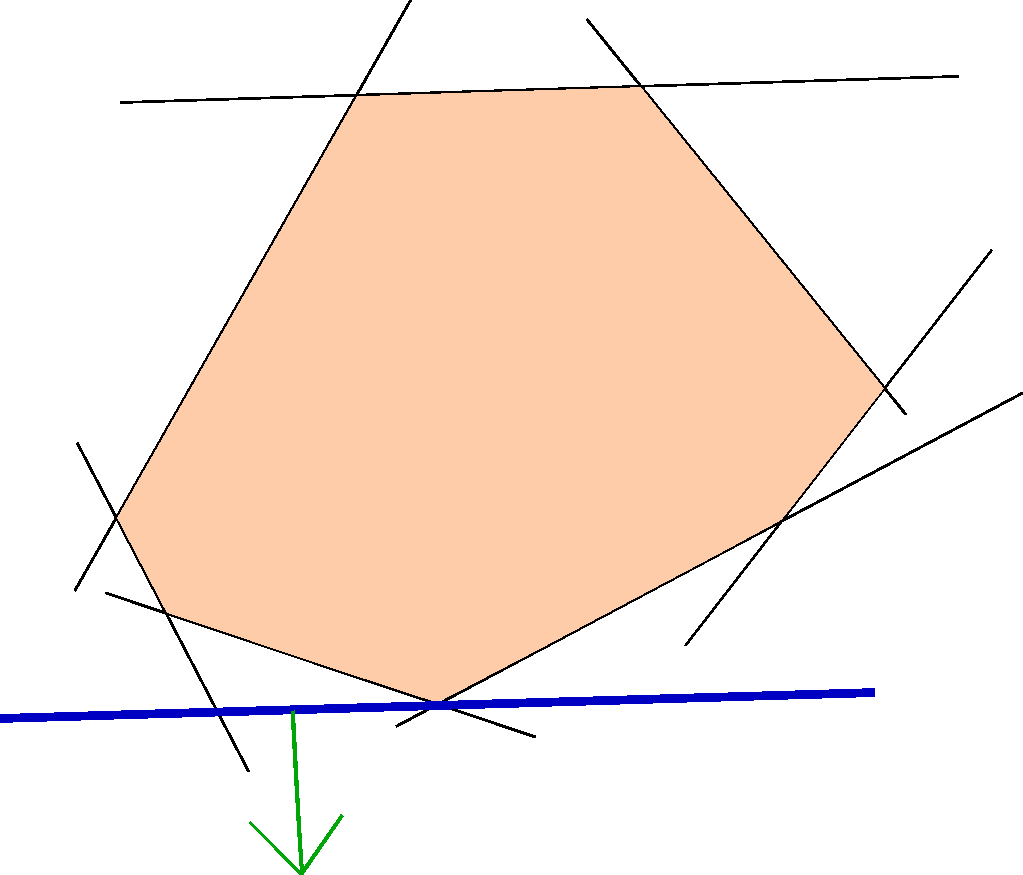
\includegraphics[width=0.65\columnwidth]{img/linopt.pdf}
		\caption[Visual representation of a 2d linear programming problem]{\textbf{Visual representation of a 2-dimensional linear programming problem.}
			The problem is constrained by seven inequalities, and the orange section represents the intersection of the half-spaces defined by these inequalities. The blue line represents the optimal isoline of the objective function (that is, all points $(x,y)\text{ s.t. }f(x,y) = o$ and $o$ is the optimum of the problem) and the green arrow the direction of the gradient (that is, the direction of the optimization). Clearly, the objective function is at its optimum on the vertex of the polygon.
		}
		\label{fig:linearprog}
	\end{figure}

	\paragraph{}
	Convex optimization is the generalization of linear programming to convex objective functions, convex inequalities and linear equality constraints.
	The search space of convex optimization problems is itself convex, as the intersection of half-spaces of convex support.
	This convexity property provide an important invariant: any local optimum is also the gloval optimum.

	\Textcite{nesterov1994interior} showed that most convex problems\footnote{Specifically linear programs, but also \emph{second order cone programs} and \emph{semidefinite programs}.}, including linear programs, can be solved in polynomial-time complexity using variations of the interior-point methods that \textcite{karmarkar1984new} introduced for linear programming.
	In general, however, convex optimization remains a NP-hard problems.%; for exemple the optimization of a quadratic objective functions subject to linear constraint, a problem in appearance easy, is a difficult problem with some instances.

	\paragraph{Approximation algorithms} a\\

	\paragraph{Optimization complexity} a\\

	\textbf{XXX PO, NPO, decision problems $\leftrightarrow$ optimization problems ($\leftarrow \exists$ solution with at most / at lest bound $b$ ; $\rightarrow$ enumerate (or binary search over) possible values of $b$) XXX}
	\phantom{oarst}a\\

	\textbf{XXX APX, FPTAS and PTAS XXX}

	\subsection{Combinatorial optimization}
	\label{subsec:combio}
	Combinatorial optimization is the large field of research interested in optimization problems defined over finite search spaces.
	That is, where the problems is to search for one optimal element inside a discrete set of objects.


	Although there exists some easy combinatorial problems, in general this is a class of problems that are often very difficult, for at least two reasons.
	\begin{enumerate}
		\item For one, even if the search space is finite, the number of feasible solutions is frequently so high that any enumeration is impossible in practice.
			For exemple in the two-sequences alignment problem.
			Given two sequences $\vec{a}=a_1a_2\ldots{}a_m$ and $\vec{b}=b_1b_2\ldots{}b_n$ ($n \leq m$) over the same alphabet, find the alignment that maximize the number of similar characters between the two alignments.
			In this problem, the number of non redundant alignments between $\vec{a}$ and $\vec{b}$ is $N(m,n)=N(m-1,n)+N(m,n-1)=\binom{m+n}{n}$ which is a clear exponential growth.

		\item Secondly, in many cases, the equivalent decision problem is itself a NP-hard problem.
			For exemple in the sequence assembly problem with the \emph{shortest superstring problem}.
			Given a set of strings $s_1, s_2, \ldots, s_n$, construct a superstring $S$ that contains all $s_i$ as substrings, and such that the length of $S$ is minimal.
			The decision problem equivalence, knowing given $s$ if there exists a superstring $S_l$ of length $l \leq s$, is actually NP-complete.
			The proof is given by a reduction of the \emph{vertex cover problem} (decision version) to this shortest superstring problem as shown by \textcite{maier1978complexity} for alphabets of size 5, and later by \textcite{raiha1981shortest} for binary alphabets.

	\end{enumerate}

	Combinatorial optimization is closely related to various algorithmic research domain both, and in particular to the complexity theory and to the combinatorics field (and any enumerative approaches).

	\begin{itemize}
		\item TSP, MST (min spanning tree)
		\item subdomain of mathematical optimization
		\item many applications
		
		\item two closely related fields, \emph{combinatorial opt.} (loosely named) and \emph{integer programming}

		\item distinction between problems for which polynomial-time algorithms exists and NP-complete problems
		\item for NP problems real-world instances (that do not exhibit difficult behavior) vs. random
		\item solving subproblem with polynomial-time algorithm (fpt algorithm..., cf)
		\item approximation

		\item For problems in P, greedy algorithms, dynamic programming, or linear programming

		\item expression as decision problem

		\item lots of categorie and subcategories

		\item \textcite{crescenzi1995compendium} published a compendium of NP opt. problems, that they maintain somewhat up to date at \parencite{npcompendium}.
	\end{itemize}

		\subsubsection{Polynomial-time solvable exemple: the min-cut problem}
		\label{subsubsec:mincut}
			\textbf{XXX Equivalent to the Max-flow problem, min-cut max-flow theorem, \textcite[Section 6.1]{papadimitriou1982combinatorial} for proof XXX}
		
		\subsubsection{Branch-and-* algorithms}
		\label{subsec:bnsalgo}

			\paragraph{Branch-and-bound}

				The branch-and-bound technique is a search space exploration technique based on the explicit traversal and pruning of the a state tree.
				It is based on the technique that \textcite{land1960automatic} applied to integer programming.

				It is very similar to the \emph{star familly} of algorithms (such as A*, B*, \dots{}) and to the \emph{alpha-beta} algorithm in regards to both space exploration and to pruning.

				\textbf{in \cref{chap:xheinz} use the min-cut algorithm introduced in \cref{subsubsec:mincut} as an heuristic}

			\paragraph{Branch-and-cut}

				The branch-and-bound algorithm requires an explicit definition of the search space for its branch operation, in order to construct the list of candidate (sub-)solutions to explore.

				Branch-and-cut is equivalent to branch-and-bound with the addition that additional constraints can be added during the execution.
				In pratice, 
				
				XXX Cannot express the whole problem (exponential number of constraints) XXX

				XXX Simply faster thanks to the addition of local cuts XXX

		\paragraph{}
		\paragraph{}
		For an introduction to optimization problems and the fundamental techniques of the domain (including Branch-and-bound methods) we recommend \textcite{papadimitriou1982combinatorial}'s classic.
		For an \emph{advanced reference} book on difficult optimization problem and their algorithms, their analysis and their precise classification, we suggest \textcite{hromkovivc2013algorithmics}'s book.
